\section{Literature Review}
%this will detail all the prior work we're building on here.
%we can say more here - both more detail and more background if needed
This section details the mathematical framework and previous research on which this project was based.

\subsection{Artificial Neural Networks}
This project uses artificial neural networks for the approximation of various functions within the agent. Artificial neural networks can be considered to be general function approximators - they learn a non-linear mapping between their inputs and outputs, the complexity of which is dependant on the hyper parameters and structure of the network.

At their most basic, a neural network consists of layers of ``neurons''. Each neuron takes a linear sum of their inputs (often the output of all the neurons in the previous layer, plus an optional bias term, but not always), then applies a non-linear ``activation function'' to that.  So the output of the jth neuron in the layer could be written as:
\begin{equation}
O_j = f\big( \sum_i (w_{ji}I_i)\big)
\end{equation} where $f(x)$ is the non-linear activation function - for example the sigmoid function, $\frac{1}{1+ \text{e}^{-x}}$.  $w_ij$ are model parameters that are learned. The non-linearity allows multiple consecutive layers to add further expressiveness to the function, and the choice of what non-linearity is used also significantly affects it's behaviour.

The two main non-linearities used within the experiments in this paper are ReLU and HardTanh. Both are non-differentiable, but do have sub-gradients. ReLU (Rectified Linear Units) are defined as:
\begin{equation}
\text{ReLU}(x) = \begin{cases}
0 & x < 0 \\
x & x \ge 0 \\
\end{cases}
\end{equation}
HardTanh are defined as:
\begin{equation}
\text{HardTanh}(x) = \begin{cases}
-1 & x < -1 \\
x & |x| < 1 \\
1 & x > 1 \\
\end{cases}
\end{equation}
Their respective advantages are that ReLU don't suffer from having a critical region where the gradients are non-zero, whilst HardTanh has the advantage that it can pass both negative and positive values.

They are trained using gradient descent to minimise the loss function of interest,which varies between applications - where a specific output is desired mean squared error is often used. The gradient of the output with respect to the input is calculated, using the backpropagation algorithm, which is essentially the chain rule applied to the consecutive layers. So for a network with layers $a, b, c$, where $O_a$ is the output of layer $a$ and $I_a$ is the input to layer $a$ then 
\begin{equation}
\frac{dL}{dI}  = \frac{dL}{dO_b} \frac{dO_b}{dO_a} \frac{dO_a}{dI} 
\end{equation} 
So the gradient can be ``back-propagated'' through the network by only considering the gradient (or sub-gradient for non-differentiable non-linearities) for the error with respect to the inputs of that layer. This then allows the gradient of the error with respect to the parameters to be easily calculated thus:
\begin{equation}
\frac{dL}{d\theta_b} = \frac{dL}{dO_b}\frac{dO_b}{d\theta_b} 
\end{equation}
which is easily done because $\frac{dL}{dO_b}$ is already known and $\frac{dO_b}{d\theta_b}$ is a calculable property of the layer. This gradient with respect to the parameters can then be used to update the parameters using standard gradient descent. This principle is shown in figure~\ref{fig:backprop}

\begin{figure}
\centering
\begin{tikzpicture}[ node distance =1cm, > =  stealth, hv path/.style={to path={-| (\tikztotarget)}}, vh path/.style={to path={|- (\tikztotarget)}},
layer/.style={ rectangle, draw, minimum width  = 1cm, minimum height = 2cm },
biglayer/.style={ rectangle, draw, minimum width  = 1cm, minimum height = 5cm }]

\node (pfeat) [layer, , label = 20: $O_a$] at(0,0){};

%circles for pfeat
\node (circ) [circle, draw, above of =  pfeat, node distance = 0.65cm] {};
\foreach \s in {1,...,3}
{
\node (circ) [circle, draw, below of = circ, node distance = 0.4cm] {};
}

\node [layer, right = of pfeat, label = 20: $O_b$] (l1) {}
	edge [<-] (pfeat);
\node (circ) [circle, draw, above of =  l1, node distance = .65cm] {};
\foreach \s in {1,...,3}
{
\node (circ) [circle, draw, below of = circ, node distance = 0.4cm] {};
}
\node [layer, right = of l1] (l2) {}
	edge [<-] (l1);
	\node (circ) [circle, draw, above of =  l2, node distance = 0.65cm] {};
\foreach \s in {1,...,3}
{
\node (circ) [circle, draw, below of = circ, node distance = 0.4cm] {};
}
\node [right = of l2] (l3) {$V_{out}$}
	edge [<-] (l2);
	
\draw [->, bend right = 60, color = blue] (l3) to node[midway, above]  (diff){\Large{$\frac{\partial L}{\partial O_b}$}} (l1.north east) ;
\draw [->, bend right = 60, color = blue] (l1.north east) to node[midway, above](diff2){\Large{$\frac{\partial O_b}{\partial O_a}$}} (pfeat.north east) ;
%\draw [->, color = blue] (diff2) to (diff);
%\node (result) [above left = of diff, color = blue] {\Large{$\frac{dL}{dO_a}$}};

\end{tikzpicture}
\caption{The Backpropagation Algorithm}
\label{fig:backprop}
\end{figure}

There are some issues with this - the key one being  that typically the error function will be non-convex, and so it is likely to get stuck in unprofitable local minima. One standard trick that help reduce that is momentum, whereby each gradient update step for the parameters also includes a weighted multiple of the previous step, encouraging it to keep going in the same direction. So the update equation becomes:
\begin{equation*}
\delta_{i,t} = \frac{dL}{d\theta_i} + m\delta_{i,t-1}
\end{equation*}
\begin{equation}
\theta_i = \theta_i  + \alpha * \delta_{i,t}
\end{equation}

The other significant problem is one of over fitting, where the neural network will start learning how to match the noise within the examples to produce an even better fit to the training data, which comes at a significant cost to it's ability to generalise. There are a number of ways to combat this, one can keep the number of parameters available to the network low, which means that it doesn't have the ability to fit the much higher order noise. However it's hard to know how large to make the network initially, and training the networks is often computationally expensive, so schemes that iteratively increase the network size take a lot of time. Two better techniques are early stopping and regularisation. In early stopping, a subset of the training data is separated, called the validation data, and after each training epoch the network is tested on the validation set. When the results on the validation set have stopped improving for some number of epochs, the training process is stopped, even if the network is still improving on the training set.

With regularisation, the norm of the parameters in each layer is limited in some way, for example by adding penalty term to the loss function for the total norm of the weights. In general with neural networks weight decay, whereby each weight is reduced by some amount after every step, or hard norm limits, whereby it scales all the parameters so that they don't exceed some limit on the norm, are used.
\subsubsection{Recurrent Neural Networks}

A recurrent neural network (RNN) is a particular architecture of an artificial neural network where a layer takes it's previous values as an input. This means that there is now a ``memory'' to the network. With a simple feed forwards network, the outputs are only a ever a function of the current input, whilst with a RNN the output is a function of all previous inputs. This means that RNNs can be used for variable length inputs or outputs. In order to train such a network, the back-propagation algorithm has to be modified to a form called ``back-propagation through time''. In this the internal states of the network are ``rolled out'', so that each previous internal state is treated as if it were a separate layer. Then the gradients for each of these rolled out layers are summed together, and this average gradient is used to update the parameters. This idea is shown in figure~\ref{fig:bptt}.

\begin{figure}
\centering
\begin{tikzpicture}[ node distance =1.3cm, > =  stealth, hv path/.style={to path={-| (\tikztotarget)}}, vh path/.style={to path={|- (\tikztotarget)}},
layer/.style={ rectangle, draw, minimum width  = 1cm, minimum height = 2cm },
biglayer/.style={ rectangle, draw, minimum width  = 1cm, minimum height = 5cm }]

\node (in1)  at (0,0) {Prior Internal State};
\coordinate [right  =of  in1] (c1);
\node (l1) [layer, above of =  c1, label  = $h_{t}$] {};
\node (i1) [left = of  l1.130, node distance = 0.8cm] {$I_{t}$};
\coordinate [right = of l1] (c2);
\node (l2) [layer, above of =  c2, label  = $h_{t+1}$] {};
\node (i2) [left = of  l2.130, node distance = 0.8cm] {$I_{t+1}$};
\coordinate [right = of l2] (c3);
\node (l3) [layer, above of =  c3, label  = $h_{t+2}$] {};
\node (i3) [left = of  l3.130, node distance = 0.8cm] {$I_{t+2}$};
\node (end) [right = of l3] {$V_{out}$}
	edge [<-] (l3);

%edges
\draw  [hv path,<-] (l1.220)to (in1);
\draw [->] (i1) to (l1.130);
\draw [->] (i2) to (l2.130);
\draw [->] (i3) to (l3.130);
\draw [->] (l1.52) to (l2.232);
\draw [->] (l2.52) to (l3.232);

%diff terms
\draw [->, bend left = 40, color = blue] (end) to node[midway, below]  (diff){\Large{$\frac{\partial L}{\partial O_{t+1}}$}} (l2.east) ;
\draw [->, bend left = 40, color = blue] (l2.south east) to node[midway, below]  (diff){\Large{$\frac{\partial O_{t+1}}{\partial O_{t}}$}} (l1.east) ;


%circles for layers
\node (circ) [circle, draw, above of = l1, node distance = 0.65cm] {};
\node (circ) [circle, draw, below of = circ, node distance = 0.4cm] {};
\node (circ) [circle, draw, below of = circ, node distance = 0.4cm] {};
\node (circ) [circle, draw, below of = circ, node distance = 0.4cm] {};
\node (circ) [circle, draw, above of =  l2, node distance =0.65 cm] {};
\foreach \s in {1,...,3}
{
\node (circ) [circle, draw, below of = circ, node distance = 0.4cm] {};
}
\node (circ) [circle, draw, above of =  l3, node distance =0.65 cm] {};
\foreach \s in {1,...,3}
{
\node (circ) [circle, draw, below of = circ, node distance = 0.4cm] {};
}
\end{tikzpicture}
\caption{Back-propagation through time}
\label{fig:bptt}
\end{figure}
More formally, the gradient with which the parameters are updated with can be considered as:
\begin{equation}
\frac{\partial L}{\partial \theta} = \sum_{1<t<T}\frac{\partial L_t}{\partial\theta}
\end{equation}
\begin{equation}
\frac{\partial L_t}{\partial\theta} = \sum_{1 < k< t} \big( \frac{\partial L_t}{\partial x_t}\frac{\partial x_t}{\partial x_k} \frac{\partial^+ x_k}{\partial\theta} \big)
\end{equation}
\begin{equation}
\frac{\partial x_t}{\partial x_k} =\sum_{t \geq i > k} \frac{\partial x_i}{\partial x_{i-1}} 
\end{equation}
 where $L_t$ is the loss at time step $t$, $x_t$ is the internal state at time $t$ and $\theta$ are the parameters of the RNN, and $\frac{\partial^+ x_k}{\partial\theta}$ is the immediate gradient of $x_k$ with respect to $\theta$. \cite{pascanu2012difficulty}
 
RNNs are very powerful, having been shown to be technically Turing complete, and are capable of handling a much broader range of situations than pure feed-forwards networks. However they have their own additional issues - they are much more prone to exploding and vanishing gradients, where the gradients of elements many steps before the reward either produce exponentially large or exponentially small gradients, either dominating any impact of more recent steps or failing to produce any learning at all for such distances. Furthermore, in part due to their power, they tend to produce chaotic responses to variations in the error surface, meaning they are much more likely to end up in unhelpful local minima.

One trick to help with the exploding gradient is to reduce the norm of the gradient of any layer before averaging to some limit by scaling down all the gradients of any layer who's gradient  norm is greater than the limit. This means that the closer points will never be dominated, which allows other hyper parameters to be set so as to reduce the vanishing gradient problem.

\subsection{Reinforcement Learning}
Reinforcement learning (RL) is ``a technique where an agent attempts to maximise it's reward by repeated interactions with a complex uncertain environment.'' \cite{Sutton:1998:IRL:551283}
RL is defined in terms of an agent working within a Markov decision process (MDP), although many applications stretch or break the definition of an MDP. An MDP is a discrete time stochastic control process, where there are some set of states the agent can be in, and in each of those states the agent can take one of a number of actions. Depending what action is chosen, the agent will transition to some state (which may be the same one) with different probabilities depending on what action was chosen, and the agent will receive some reward depending on what transition happened. An important property of an MDP is that it is Markovian, that is that what actions can be taken and the transition probabilities are solely a function of the current state, no matter what route was taken to get there or anything else like that. One such process is displayed in figure~\ref{fig:mdpsimple}

\begin{figure}
\centering
\begin{tikzpicture}[ node distance = 2cm, > =  stealth,
%define the style for each of the nodes here
state/.style={
% The shape:
circle,minimum size=14mm,
% The rest
very thick,draw=black!60, text = black!90,
top color=white,bottom color=black!20},
%the style for the highlighted node - change the term in square brackets to this to change the node to this
action/.style={
% The shape:
rectangle,minimum size=9mm,rounded corners=2mm,
% The rest
very thick,draw=black!50,
top color=yellow!10,bottom color=yellow!40},
%the style for the info boxes on the right
info/.style={
% The shape:
rectangle,minimum size=6mm,rounded corners=2mm,
%text width and the bullet points
 text width = 3.5cm,
% The rest
very thick,draw=black!40,
top color=white,bottom color=yellow!20}
]
%create the nodes and link them with arrows
\node (A) [state] at (0,0) {A};
\node (a1) [action, right of =  A, label ={[blue]5: 0.3}, label  = {[blue]273: 0.7}] {$a_1$}
	edge [<-] (A);
\node (a2) [action, above right of  = A, label ={[blue] 10: 1}] {$a_2$}
	edge [<-] (A);
\node (B) [state, right = of a1] {B}
	edge [<-] node [midway, above] {$r_1$}(a1)
	edge [<-, bend right] node [midway, above] {$r_2$}(a2);
\node (b1) [action, above right of = B, label = {[blue]85: 0.4}, label  ={[blue] 283: 0.6}] {$a_3$}
	edge [<-] (B);

\draw (a1.south) [->,bend left = 80] to node [midway, below] {$r_3$} (A); 
\draw (b1.north) [->, out = 120, in = 90] to node [midway, above] {$r_4$} (A); 
\draw (b1.290) [->, out = 270, in = 0] to node [midway, right] {$r_5$} (B); 
	
\end{tikzpicture}
\caption{A markov decision process}
\label{fig:mdpsimple}
\end{figure}

A reinforcement learning agent is primarily concerned with estimating two functions: the Value function and the Q function, which are shown in figure~\ref{fig:rlsimple}, based on the policy, $\pi$ it is assessing. The policy determines what action is chosen in each state. The value function is a function of state, which estimates the expected reward that the agent would receive continuing to follow $\pi$ from that state. The Q function is a function of state and action, which estimates  the expected reward the agent would receive if it were to return to following $\pi$ after taking that action in that state.

\begin{figure}
\centering
\begin{tikzpicture}[ node distance = 1cm, > =  stealth,
%define the style for each of the nodes here
stage/.style={
% The shape:
rectangle,minimum size=6mm,rounded corners=2mm,
% The rest
very thick,draw=black!50, text = black!90,
top color=white,bottom color=black!20},
%the style for the highlighted node - change the term in square brackets to this to change the node to this
highlight/.style={
% The shape:
rectangle,minimum size=6mm,rounded corners=2mm,
% The rest
very thick,draw=black!50,
top color=yellow!10,bottom color=yellow!40},
%the style for the info boxes on the right
info/.style={
% The shape:
rectangle,minimum size=6mm,rounded corners=2mm,
%text width and the bullet points
 text width = 3.5cm,
% The rest
very thick,draw=black!40,
top color=white,bottom color=yellow!20}
]
%create the nodes and link them with arrows
\node (start) [stage, label = V] at (0,0){State};
\node (s2) [highlight] [right = of start, label = Q] {Action}
	edge [<-] (start);
\node (s3) [stage] [below =  of s2] {Environment}
	edge [<-](s2)
	edge [->,bend left = 40] node[left] {reward} (start);
	
\end{tikzpicture}
\caption{A simplified view of the Reinforcement learning problem}
\label{fig:rlsimple}
\end{figure}

Reinforcement learning can be used for policy evaluation, where V and Q are estimated for the given policy $\pi$, though that requires the policy to have been explicitly defined elsewhere. This is done by running the agent and updating the estimates until convergence. In order for it to produce an estimate for every V and Q it has to visit each state and action an unbounded number of times. However, often what is desired is the discovery of the optimal policy $\pi^*$. This can be found by a process called policy iteration. In policy iteration some initial policy is chosen, then evaluated, then improved using the information from the evaluation, then the improved policy is evaluated and the process repeated until convergence. Often it is expedient to not wait for the policy evaluation to converge, but rather perform partial steps of both the evaluation and the improvement. These smaller steps often lead to much faster convergence, provided it still is able to visit every state.

A RL agent can either  be following the policy it is evaluating, in which is called an on-policy method, or it can be following a different policy to the one it is evaluating, called an off policy method. On policy methods are simpler, but require the policy to naturally explore the whole state space. Depending on the situation, it is often desirable to have a final policy that doesn't do the exploration on it's own, in which case an off policy method would be required.

\subsubsection{Temporal Difference Methods}
Temporal difference methods are all based on using the bellman step to update the estimates of V(s) and Q(s,a) after every transition.
\begin{equation}
V(s_n) \gets r + \gamma V(s_{n+1})
\end{equation}
$\gamma < 1$ is a constant that discounts future rewards, so that for environments with unbounded episode length the value function remains finite. There are several methods to estimate the Q function - the two key ones are SARSA and Q-Learning.

SARSA is an on-policy algorithm which assesses the policy it is following. It follows an update step of:
\begin{equation}
Q(s_n,a_n) \gets r + \gamma Q(s_{n+1}, a_{n+1}) 
\end{equation}
Where $a_n$ is the action chosen by $\pi$ at step $n$. As this is an on-policy algorithm, $\pi$ has to be sufficiently exploratory. When performing policy iteration, the normal procedure is to make $\pi$ greedy with respect to the calculated Q values. But this won't explore enough on it's own, so in addition, $\pi$ is modified so that it has a small chance $\epsilon$ to take a random action on any step. This ``epsilon greedy'' algorithm is detailed in figure~\ref{alg:epsgreedy}. After each Temporal difference update to the Q function, the policy is effectively updated in that region.

\begin{figure}
\centering
\begin{algorithmic}
\State In state $s$, with available actions $\boldsymbol{a}$
\WithP[$\epsilon$]
	\State Choose $a$ from $\boldsymbol{a}$ with uniform probability
	\State Perform action $a$
\ElseP
	\For{ each $a$ in $\boldsymbol{a}$}
		\State Evaluate Q($s,a$)
		\If{ Q($s,a) > $Q$_{max}$}
			\State Q$_{max} \gets $ Q($s,a$)
			\State $a_{max} \gets a$
		\EndIf
	\EndFor
	\State Perform action $a_{max}$
\EndP
\end{algorithmic}
\caption{Epsilon greedy policies}
\label{alg:epsgreedy}
\end{figure}

Q learning also uses an epsilon greedy policy to choose it's actions, however Q learning is an off policy algorithm, which actually learns about the purely greedy policy. In Q learning the update for Q is:
\begin{equation}
Q(s_n,a_n) \gets r + \gamma \max_a \{Q(s_{n+1}, a) \}
\end{equation}
The max term ensures that, no matter what action is actually chosen in the next state, it learns about the value if it were following the purely greedy policy.

These two algorithms converge to fundamentally different policies, even if we base a purely greedy policy on the final output of SARSA, as a simple example will show. In the simple grid world in figure~\ref{fig:gridworld} there is a start, a goal and a cliff. The agent starts at the start, can always choose to move in cardinal directions, gets a reward of 1 for getting to the goal, -1 for stepping off the cliff, both of which end the episode, and  a reward of -0.01 otherwise. The two agents converge to the different policies shown in figure~\ref{fig:gridworldpaths}. Because the SARSA agent learns on policy, it learns a policy that takes account of the random steps it takes, and so ends up travelling further away from the cliff edge. On the other hand the Q-Learning agent only learns about the states as if it always follows the greedy action, so the Q learning agent travels right up against the cliff edge, as that is the optimal path if it always takes greedy actions.

\begin{figure}
\begin{subfigure}{0.5\textwidth}
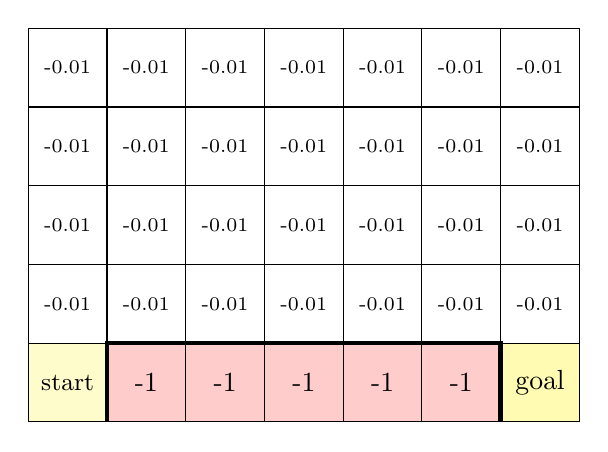
\begin{tikzpicture}[ node distance =1.3cm, > =  stealth, hv path/.style={to path={-| (\tikztotarget)}}, vh path/.style={to path={|- (\tikztotarget)}}]

\foreach \x in {1,...,7} 
{
	\foreach \y in {2,...,5} 
	{
	\node [rectangle, draw, minimum size = 1cm] at (\x,\y) {\scriptsize{-0.01}};
	}
}
\node [rectangle, draw, minimum size = 1cm, fill = yellow!20] at (1,1) {};
\node at (1,1) {\small{start}};
\node [rectangle, draw, minimum size = 1cm, fill = yellow!30] at (7,1) {goal};
\foreach \x in {2,...,6} 
	{
	\node [rectangle, draw, minimum size = 1cm, fill = red!20] at (\x,1) {-1};
	}
%cliff border	
\draw [ultra thick] (1.5, 0.5) -- (1.5,1.5) -- (6.5,1.5) -- (6.5,0.5);
\end{tikzpicture}
\caption{The gridworld}
\label{fig:gridworld}
\end{subfigure}
\begin{subfigure}{0.5\textwidth}
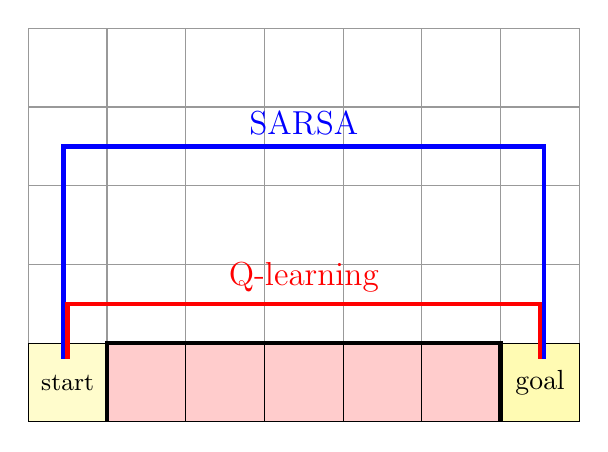
\begin{tikzpicture}[ node distance =1.3cm, > =  stealth, hv path/.style={to path={-| (\tikztotarget)}}, vh path/.style={to path={|- (\tikztotarget)}}]

\foreach \x in {1,...,7} 
{
	\foreach \y in {2,...,5} 
	{
	\node [rectangle, draw, minimum size = 1cm, black!40] at (\x,\y) {};
	}
}
\node [rectangle, draw, minimum size = 1cm, fill = yellow!20] at (1,1) {};
\node at (1,1) {\small{start}};
\node [rectangle, draw, minimum size = 1cm, fill = yellow!30] at (7,1) {goal};
\foreach \x in {2,...,6} 
	{
	\node [rectangle, draw, minimum size = 1cm, fill = red!20] at (\x,1) {};
	}
%cliff border	
\draw [ultra thick] (1.5, 0.5) -- (1.5,1.5) -- (6.5,1.5) -- (6.5,0.5);
%SARSA path
\draw [ultra thick, blue] (0.95,1.3) -- (0.95,4) -- node[midway, above] {\large{SARSA}} (7.05,4) -- (7.05,1.3);
%Q-learning path
\draw [ultra thick, red] (1,1.3) -- (1,2) -- node[midway, above] {\large{Q-learning}} (7,2) -- (7,1.3);
\end{tikzpicture}
\caption{The paths taken by the agents}
\label{fig:gridworldpaths}
\end{subfigure}
\caption{A demonstration of the difference in pathing for SARSA and Q-learning}
\end{figure}

\subsection{Function Approximators}
So far all of the above maths has implicitly been assuming that V(s) and Q(s,a) are actually looking up values from a table, such that the function can take any arbitrary value for any of the states and actions. For many applications this is unrealistic - it requires the agent to be able to experience every possible state during training to learn the values for them, which may not be possible for practical reasons and in any case is computationally prohibitive. Far preferable would be to use some function approximation to V(s) and Q(s,a) that could generalise from the experiences it has had to those it hasn't.

There are several key challenges this brings up however: ones of stability, generalisation and expressiveness. If the function isn't expressive enough to describe the optimal policy then the agent will converge to a suboptimal policy, if at all. In general there is no guarantee that the function will converge, and often it may well diverge - in particular there are issues where the initial errors in estimates for the Q values of local states can be amplified by the local updates due to the spreading from the function approximation. This can be reduced by sticking to linear function approximators, but then there are issues with the expressiveness. Lastly, the feature set chosen for the function approximators needs to be able to generalise sufficiently whilst also being able to tell the difference between good and bad states.

One other interesting impact of using a function approximation is that, because by it's nature the function approximation can't produce the true Q value everywhere, it's most desirable for it to be correct in states where the agent is likely to travel, whilst wrong about states that the agent shouldn't end up in. So although it still needs to be able to explore every state to check to see what are better, more of the learning effort should be focussed on more profitable states.

Because of those reasons, for many years it was considered impossible to use neural networks as the function approximators in reinforcement learning. However, in \cite{atariDQN} the team at Google Deepmind managed to train a deep network to play Atari games using reinforcement learning. The key changes are that they used experience replay and a target network. 

With experience replay they store a set of the previous transitions, then at each learning step, rather than just update with the last transition, they produce a mini-batch of a random selection of previous transitions to learn from, and apply Q-learning for each of them to create the targets to update the network weights with. The randomness helps reduce the chance of the network ``forgetting'' something that it learned from a previous transition and helps improve learning stability. 

The target network is a copy of the network that evaluated the Q values  but with different weights. In their implementation they copied across their weights to the target network after a large fixed number of steps. The target network was used in the update steps in place of the Q network values for producing the value of the next state, as follows, where $\theta$ is the network weights and $\theta'$ are the target network weights :
\begin{equation*}
L(s,a) = (Q(s,a;\theta) - (r + \gamma Q(s,a; \theta' )))^2
\end{equation*}
\begin{equation}
\theta = \theta + \alpha \frac{\partial L}{\partial \theta}
\end{equation}

\subsubsection{Policy Gradient Methods}
In many applications of reinforcement learning, it is necessary to deal with continuous state and action spaces. This is a departure from the strict definition of a Markov decision process, but in many cases sufficient discretization leads to intractably large state and action spaces anyway. In such cases both Q learning and SARSA face issues due to the need to calculate the maximum of an arbitrary function at each action step. Instead what is used is some policy function $\pi(s;\theta)$ which outputs the continuous action $a$ for any particular step. Then this policy is updated after some number of steps based on the gradient of the expected total rewards with respect to the parameters. This expectation is notated as $J(\theta)$, and is defined as:
\begin{equation}
J(\theta) = \mathbb{E}\big[\sum_t=1^T r_t \big] = \mathbb{E}[R]
\end{equation}

In REINFORCE the sample approximation to this gradient is formed as, after running through M episodes:
\begin{equation}
\nabla_\theta J = \frac{1}{M}\sum_{i=1}^M\sum_{t=1}^T\nabla_\theta  \text{log}\pi ( s_{1:t}^i ; \theta)(R^i_t - b_t)
\label{eq:Reinforce}
\end{equation}
This is produced by approximating the action value function as if it were the sample return.

This method is again on-policy, and indeed only works for stochastic policies, as the log trick used to remove the dependence on the gradient of state distribution from the performance gradient depends on the policy having a non-zero probability of taking any action. Indeed, for a long time it was thought that in order to calculate the policy gradient for a deterministic policy a model of the environment is needed to work out the state distribution.

However, in \cite{silver2014deterministic}, it was shown that, providing some basic properties of the function are true, the gradient of a deterministic policy $\mu(s)$ is:
\begin{equation}
\nabla_\theta J =\mathbb{E}\big[ \nabla_\theta  \mu ( s ; \theta^\mu) \nabla Q^\mu (s,a)|_{a = \mu(s)}\big]
\end{equation}
This can be implemented using an Actor-Critic method, whereby there is a separate actor and critic networks, the actor implementing $\mu$ and the critic $Q^\mu$. The actors weights are updated according to the above gradient, whilst the critic can use SARSA or Q learning updates as in the discrete case, but taking action as an input.

In \cite{lillicrap2015continuous} the above was combined with the insights from \cite{atariDQN} to produce an actor critic system that used the deterministic policy gradient to train deep neural networks to produce the control for various continuous tasks. The main additional innovation was that the target network parameters are slowly updated towards the current parameters at each step, rather than copying across after some number of steps, to better keep the systems disjoint.

\subsection{Related Work}
In \cite{ling2016latent} %read the actual paper and rewrite this bit please
google deeepmind look at the parsing and analysis of Magic: the Gathering cards using deep networks, which is a crucial step in developing a competent AI to play the game as a whole.

In \cite{alphaGo} the team at Google Deepmind produced an agent trained by reinforcement learning that beat the world champion at the board game Go. There are many interesting developments on the standard RL trained model, such as retaining a smaller network for their monte-carlo tree searches, but the most interesting technique for this paper was their method of initially training the agent. They first taught the agent to predict expert moves from a large series of board states in a supervised manner. Having trained this agent, the same networks were then used to initialise a reinforcement learning agent that they then played against itself for an extended period of time to produce the value network with which they made the initial decisions with the AlphaGo agent. 
%what is the related work to the results of this project?

